\begin{figure}[t]
\centering
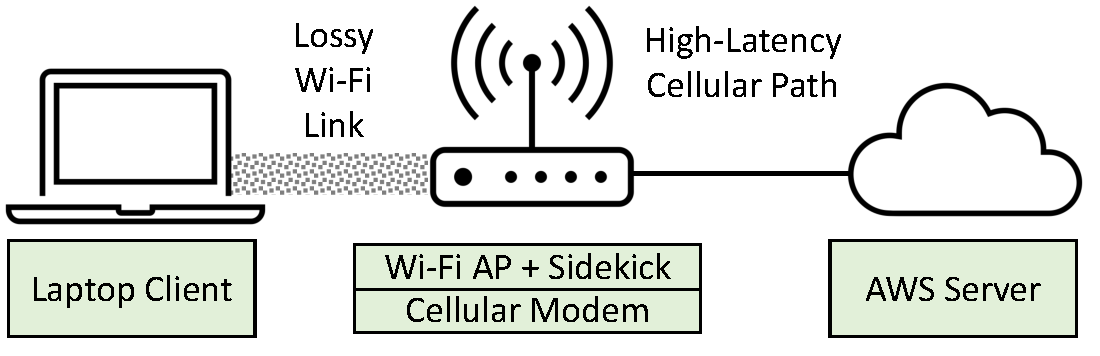
\includegraphics[width=\linewidth]{sidekick-paper/figures/setup_real.pdf}
\caption{Real-world experimental setup.
\vspace{-0.4cm}
}
\label{fig:setup:real}
\end{figure}


\section{Evaluation}
\label{sec:evaluation}

\begin{figure*}
\begin{subfigure}{0.34\textwidth}
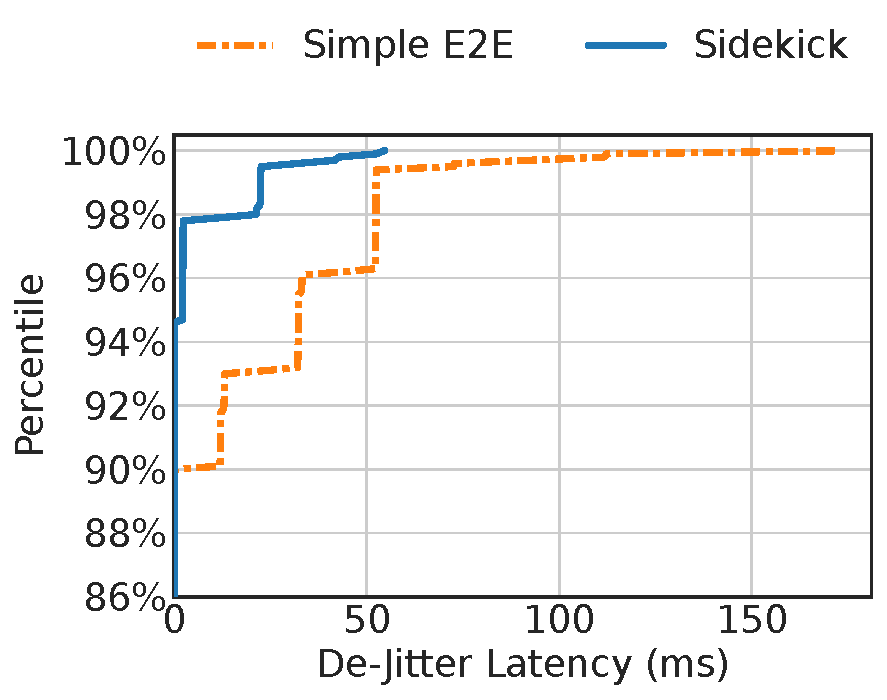
\includegraphics[width=\linewidth]{sidekick/figures/fig4a_low_latency_media.pdf}
\caption{Scenario \#1: Low-latency media.
 Reduced tail latency of de-jitter delay
with earlier retransmission. 5 minute trials.}
\label{fig:sidekick:main-results:media}
\end{subfigure}
\hfill
\begin{subfigure}{0.31\textwidth}
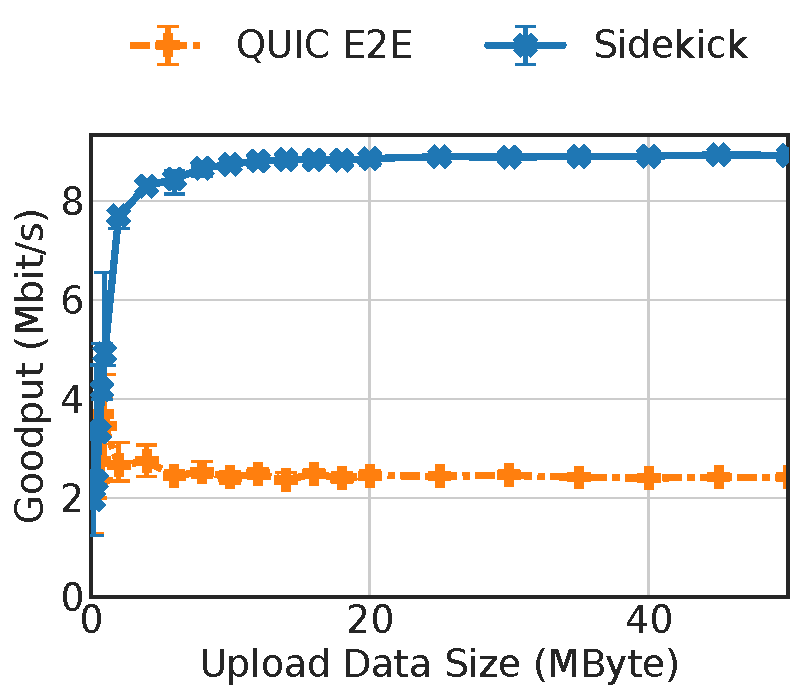
\includegraphics[width=0.97\linewidth]{sidekick/figures/fig4b_pep_emulation.pdf}
\caption{Scenario \#2: Connection-splitting PEP emulation. Improved goodput.
20 trials median. Error bars are 1st and 3rd quartiles.
}
\label{fig:sidekick:main-results:pep-emulation}
\end{subfigure}
\hfill
\begin{subfigure}{0.32\textwidth}
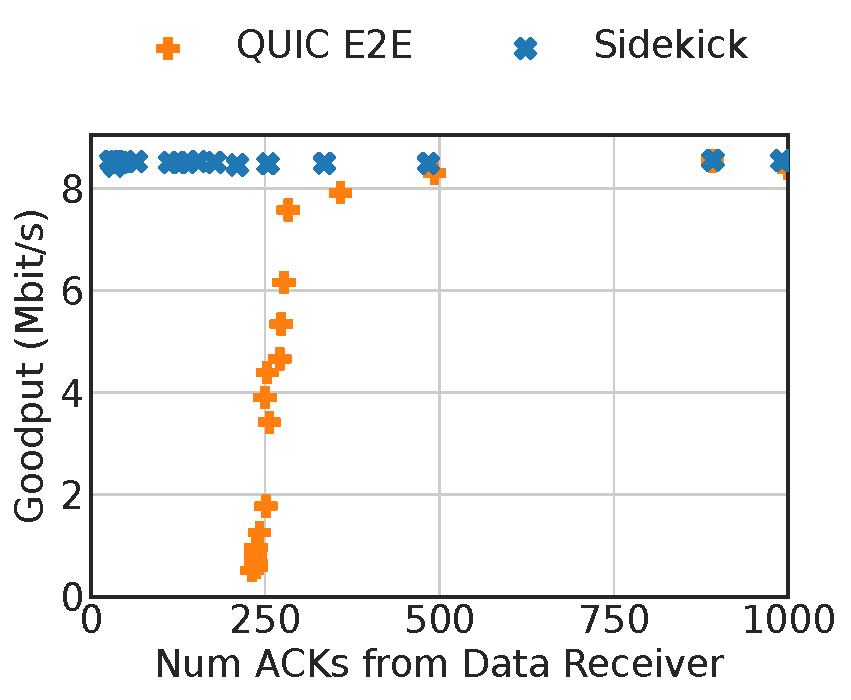
\includegraphics[width=0.99\linewidth]{sidekick/figures/fig4c_ack_reduction.pdf}
\caption{Scenario \#3: ACK reduction.
High goodput independent of end-to-end ACK frequency.
10 MB upload.}
\label{fig:sidekick:main-results:ack-reduction}
\end{subfigure}
\caption{
Comparing the end-to-end baseline protocol to the same protocol with a Sidekick
connection, using the success metrics for the three scenarios described in
\Cref{tab:sidekick:experimental-scenarios}. The \textsf{Sidekick($N$x)} data points show
the performance at $N$x the quACK interval (sent less frequently) and
threshold of the default configurations specified in
\Cref{tab:sidekick:experimental-scenarios}.
}
% \dm{Maybe a notation like $x/4$ would be more suggestive than $4x$?}
\label{fig:sidekick:main-results}
\end{figure*}


We evaluated Robin to answer the following questions:
\begin{enumerate}[noitemsep,topsep=0pt]
	\item Can {\sys}s improve the performance of opaque transport protocols
	in a variety of scenarios while preserving the opaque behavior of the
	base protocols?
	\item Can a path-aware congestion control algorithm match the fairness of
	split TCP PEPs using CUBIC?
	\item How do the CPU overheads of encoding quACKs impact the maximum
	capacity of a proxy with a \sys?
	\item What link overheads does the power sum quACK add and how does it
	compare to the strawmen?
	\item Is Robin robust in a real-world environment?
\end{enumerate}

% The goal of our evaluation is to show that \sys protocols with quACKs can
% enable performance enhancements, for an end-to-end encrypted protocol, that
% would have resulted in ossification for TCP. We evaluate QUIC using the \sys
% protocol for client-side retransmission in a scenario where TCP and QUIC both
% perform poorly without assistance from a proxy. We demonstrate the validity of
% our comparisons by further analyzing the behavior of these protocols both with
% and without assistance, and that the performance improvements we saw in quACKs
% still result in multi-flow fairness.

\subsection{Experimental Setup}

We modeled the scenarios from \Cref{sec:motivation} in both
emulated and real-world environments. We answer questions 1-4 in emulation
and question 5 in the real world. We use the same m4.xlarge AWS instance
as before for the emulated experiments, and as the server in the real-world
experiments.

\paragraph{Emulated environment.}
We emulated a two-hop network topology (\Cref{fig:sc-protocols}) in mininet,
configuring the link properties using \texttt{tc}.
In emulation, we represented
each link by a constant delay (with variability induced by the queue), a random
loss percentage, and a maximum bandwidth.
\Cref{tab:experimental-scenarios} describes the parameters
for each link to model---e.g., lossy Wi-Fi or a high-latency cellular
path---as well as the metrics for success in that scenario.
Link 1 connects the data sender (client) to the proxy,
while Link 2 connects the proxy to the data receiver (server).
On the proxy, we either run a \sys,
a connection-splitting TCP PEP~\cite{caini2006pepsal}, or nothing at all.

\paragraph{Real-world environment.}
To test its robustness, we also evaluated Robin over a real-world
environment that resembled the scenario on the train (\Cref{fig:setup:real}).
In this setup, a Lenovo ThinkPad laptop, running Ubuntu 22.04.3 with a 4-Core
Intel i7 CPU @ 2.60 GHz and 16 GB memory, acted as a client to an AWS instance in
the nearest geographical region. The ThinkPad used as an access point (AP)
a Lenovo Yoga laptop, running Ubuntu 20.04.6 with a 4-Core Intel i5 CPU @
1.60 GHz and 4 GB memory, with a 2.4 GHz Wi-Fi hotspot.
The AP was connected to the Internet via a JEXtream cellular modem
with a 5G data plan. The AP ran \sys software.

We measured the link properties of each path segment to compare to
our emulation parameters. We measured delay and loss using 1000~\texttt{ping}s
over a 100 second period, and bandwidth using an \texttt{iperf3} test.
On the near segment between the ThinkPad client and the AP,
the min/avg/max/stdev RTT was 1.249/37.194/272.168/54.660 ms
at 49.8 Mbit/s bandwidth. We observed that loss increased
the further away the AP. In our experiments, the client was located roughly
200 feet away in a different room, with 3.6\% loss.
The far segment between the AP and the AWS server was
48.546/64.381/92.374/6.806 ms with 0.0\% loss at 30.9 Mbit/s.
In both environments, the cellular link was the bottleneck link in terms of
bandwidth, and the corresponding path segments in emulation had similar
minimum RTTs and average loss percentages.

\subsection{Performance Comparison to Baseline}

We first evaluate Robin's main performance goal: In each of the motivating
scenarios, we show that Robin can improve performance compared to the base
protocol alone, which would not be able to benefit from existing PEPs.
Each scenario has a different metric for success---tail latency, throughput,
or number of packets sent by the data receiver (corresponding to energy usage
or chance of Wi-Fi collisions)---demonstrating the versatility of the \sys
protocol.

% In Scenario 1, we quACK very frequently in order to
% minimize the additional time required to detect a loss. In Scenario 2, we
% quACK just often enough so that the client can detect loss on the near path segment
% via the quACK before the end-to-end mechanism. In Scenario 3, we quACK more
% frequently with a higher threshold because the quACKs are the main signal of
% loss over the entire connection, including congestive loss at the proxy queue.

\paragraph{Low-Latency Media.}
The \sys can reduce tail latencies in a low-latency media stream, representing
fewer drops and better quality of experience.
The early retransmissions induced by the \sys reduced the 99th percentile
latency of the de-jitter buffer delay from 48.6 ms to 2.2 ms---a 95\%
reduction (\Cref{fig:media}).
% Effects of the \sys protocol for lossier networks are longer end-to-end RTTs.
% 2.240 / 48.557 = 4.6%
% 48.557 / 2.240 = 21.7x
% It improves the p95 latency by XX\%.
As long as the quACK interval is less than the end-to-end RTT, the connection
benefits from the \sys.

The \sys is beneficial in this scenario because it enables the client to sooner
detect and retransmit lost packets, and the server to sooner play packets from
its de-jitter buffer.
The end-to-end mechanism takes one additional received packet to notify of the
loss and
one end-to-end RTT to retransmit and play the packet (20+52=72ms), resulting in
three delayed packets (the three ``steps" in \Cref{fig:media}) in most cases.
The \sys takes up to two additional packets and one near path segment RTT
(20+2=22ms or 20$\times$2+2=42ms), delaying either one or two packets in comparison.
Dropped ACKs and quACKs account for the $<2\%$ of packets with even greater
de-jitter latencies.

\paragraph{Connection-Splitting PEP Emulation.}
% data['quack_30ms_10'][0][14] = 10.0
% data['quack_30ms_10'][1][14] --> median 1.093 MB/s, mean 1.091 MB/s
% data['quic'][1][14]          --> median 0.307 MB/s, mean 0.305 MB/s
% improvements							  3.560x           3.577x
The \sys improves upload speeds when there is a lossy, low-latency link
by using quACKs to inform the sender's congestion control.
In a scenario with $1\%$ random loss on the link between the proxy and the
data sender, the HTTP/3 (QUIC) client achieves $3.6\times$ the goodput for a 10 MB
upload with a \sys compared to end-to-end QUIC (\Cref{fig:baseline-line}).
% Note in this scenario, the end host also retransmits lost packets,
% but does not move the flow-control window, in response to quACKs.

When there is no random loss, the \sys does not impact the performance
of QUIC\@.
There are no logical changes to the base protocol in this case because all loss
is on the
bottleneck link on the far path segment, and the CPU overheads of processing quACKs
are negligible.

Knowing \emph{where} congestion occurs is an opportunity for creating smarter
congestion control.
In PACUBIC, identifying where the loss occured let the data sender
reduce the congestion window proportionally to how many packets were in-flight
on each path segment.
In \Cref{sec:eval:pep-comparison}, we will show that our
path-aware congestion control algorithm still matches the fairness of
connection-splitting TCP PEPs.

\paragraph{ACK Reduction.}

% min_ack_delay.py
%
% ylabel = 'h1-eth0 tx_packets'
% xs = [0, 1, 2, 3, 4, 5, 6, 7, 8, 9, 10, 20, 30, 40, 50, 60, 70, 80, 90, 100, 200, 300, 400, 500, 600, 700, 800]
% ys_quack = [7459.1, 7358.9, 3884.1, 2596.9, 1967, 1583.666, 1483.333, ???.?, ????.?, 992,   890, 481.833, 334.5, 251.6, 207.2,   177.4, 153,   138.285, 124.4, 113.2, 65.3, 50,    42.1,  36.4,  33.9,  31.6,    29.7]
% ys_quic =  [7458.9, 7403.9, 3882.9, 2600.1, 1987, 1592.9,   1498.4,  1318.9, 1131.5, 993.3, 890, 492,     356.1, 278.1, 308.777, 266.7, 257.8, 246.6*,  241.8, 248.2, 246, 242.3, 241.8, 237.1, 234.7, 233.777, 231]
%
% ylabel = 'Goodput (Mbit/s)'
% ys_quack = [8.645, 8.627, 8.633, 8.624, 8.628, 8.613, 8.599, ?.???, ?,???, 8.526, 8.570,  8.535, 8.505, 8.566, 8.572, 8.533, 8.575, 8.430, 8.591, 8.493, 8.458, 8.481, 8.332, 8.569, 8.335, 8.217, 8.291]
% ys_quic =  [8.647, 8.646, 8.632, 8.623, 8.473, 8.497, 8.559, 8.545, 8.549, 8.488, 8.523*, 8.314, 7.961, 7.734, 5.608, 5.501, 4.931, 4.488*, 4.067, 3.540, 1.818, 1.252, 0.952, 0.783, 0.665, 0.578, 0.519]

% max quack goodput before it starts declining is 8.569 Mbit/s at 500ms freq
% min number of tx_packets is 36.4 for freqs <= 500ms, min goodput is 8.333
% min_ack_delay for quic with equivalent goodput is 10ms. 8.523 Mbit/s.
% min number of tx_packets is 890.
% 36.4 / 890 = 4.1% of the packets
% 890 / 36.4 = 24.45

Using quACKs in lieu of end-to-end ACKs allows the data receiver to
significantly reduce its ACK frequency while maintaining high goodput.
% Studies show that sending ACKs less frequently can save energy in low-powered
% devices and improve performance by reducing collisions or contention for
% half-duplex links such as Wi-Fi~\cite{custura2023reducing,li2020tack}.
In our experiment, QUIC with a \sys sent $96\%$ fewer packets (mainly ACKs)
than end-to-end QUIC before the goodput dropped below 8.5 Mbit/s
(\Cref{fig:ack-reduction}).
The quACK enables the data sender to promptly move the flow-control window forward,
as long as the last hop is reliable.

The goodput significantly degrades when reducing the end-to-end ACK frequency
without a \sys. When end-to-end QUIC reduces the ACK frequency to every
80 ms, the data receiver sends $247 / 138 = 1.8\times$ the packets at
$4.5 / 8.4 = 0.5\times$ the goodput, worse than QUIC with the \sys
in both dimensions (\Cref{fig:ack-reduction}). With a \sys,
% num pkts gput  proto
% 138.285  8.430 quack
% 246.6    4.488 quic
% 246.6/138.285 = 1.8x
% 4.488/8.430 = 0.5x
the data sender also does not need to change packet pacing to avoid bursts in
response to infrequent ACKs, which is why end-to-end QUIC cannot send fewer
than $\approx 240$ packets.

\subsubsection{Configuring the \Sys Connection}
\Cref{tab:experimental-scenarios} shows the quACK interval and threshold we
elected for each scenario based on the considerations in
\Cref{sec:design:configuration}. In each experiment in \Cref{fig:main-results},
we also show how with
less frequent quACKs ($2\times$ and $4\times$ the interval) and
proportionally-adjusted thresholds, the protocol performs worse, or more
variably.
Less frequent quACKs means the client reacts later to feedback about
the near path segment, and more often has to rely on the end-to-end mechanism.
The performance particularly degrades when the quACK interval exceeds the
end-to-end RTT.
%
% \dm{This seems plausible, but does the data show this, or is it
% possible that the E2E mechanism does not get invoked more often but
% the difference is explained by waiting longer for the quACKs?  Also,
% is 4 a magic number because of 3 duplicate Acks, or would be same be
% true of 3x, or some sort of hybrid packet count and time-delay quACK?}
% We don't use 3-dupack to detect loss, just any unordered packets.
%
However, even in this case, the base protocol with any \sys at all performs
better than the base protocol alone\@.

\subsection{Fairness Evaluation}
\label{sec:eval:pep-comparison}

\begin{figure}[t]
\centering

\includegraphics[width=\columnwidth]{figures/fig5_baseline_bar_legend.pdf}
\begin{subfigure}{0.49\linewidth}
	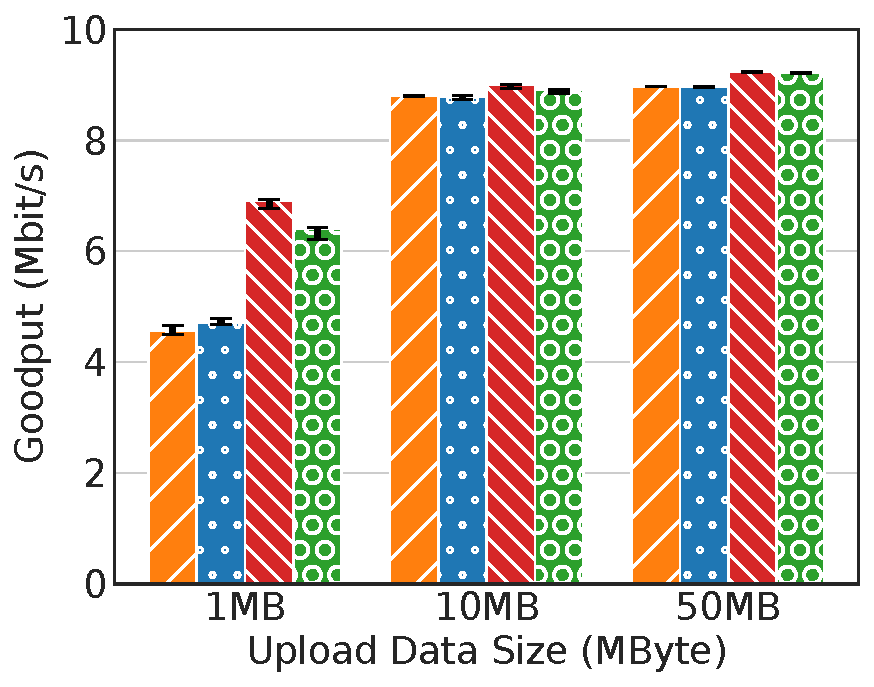
\includegraphics[width=\linewidth]{figures/fig5_baseline_loss0p.pdf}
	\caption{0\% loss.}
	\label{fig:baseline-bar:loss0p}
\end{subfigure}
\begin{subfigure}{0.49\linewidth}
	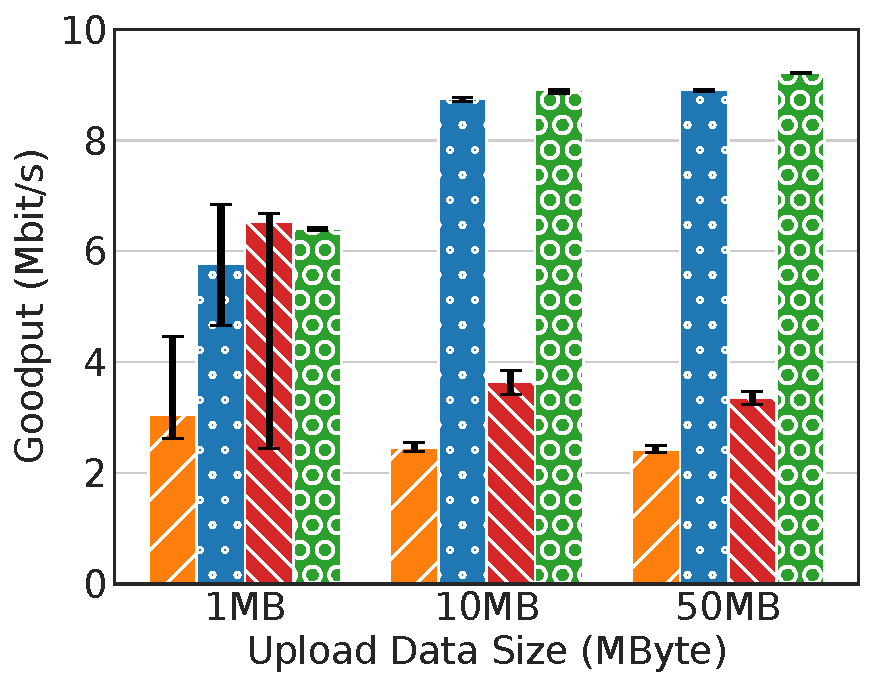
\includegraphics[width=\linewidth]{figures/fig5_baseline_loss1p.pdf}
	\caption{1\% loss.}
	\label{fig:baseline-bar:loss1p}
\end{subfigure}
\vspace{-0.2cm}
\caption{Median goodput for three upload data sizes with $0\%$ and $1\%$ loss on
Link 1. 20 trials. Error bars are 1st and 3rd quartiles.
With proxy assistance at $1\%$
loss, both QUIC and TCP match the performance of when there is no loss at all.
\vspace{-0.4cm}
}
\label{fig:baseline-bar}
\end{figure}

\begin{figure}[t]
\centering
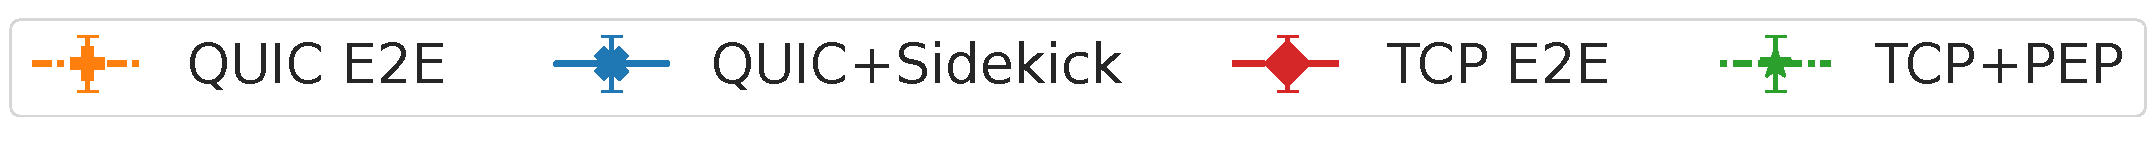
\includegraphics[width=\columnwidth]{figures/fig6_legend.pdf}
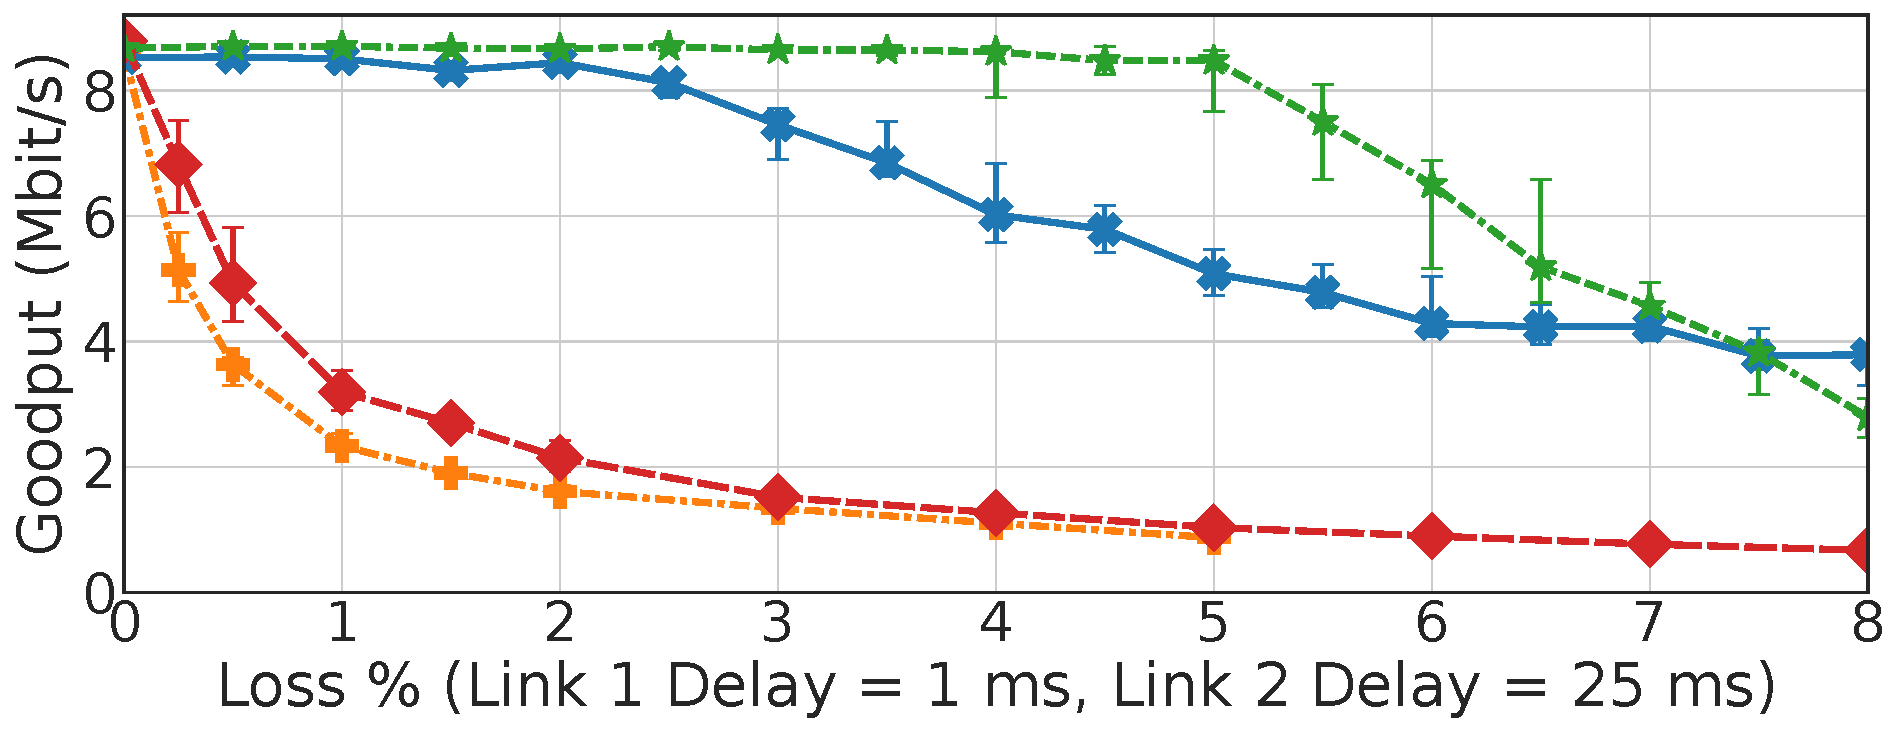
\includegraphics[width=\columnwidth]{figures/fig6_loss_bw100_10M_delay_25ms_1ms.pdf}
%\includegraphics[width=\columnwidth]{figures/loss_bw100_10M_delay_15ms_11ms.pdf}
\vspace{-0.4cm}
\caption{Connection-splitting PEP emulation as a function of near-segment
	loss rate. In this emulation experiment, QUIC+\Sys (running PACUBIC)
  performs similarly to TCP+PEP (each connection running CUBIC)
  and improves goodput compared with end-to-end protocols. The graph shows
  median goodput of a 10~MByte upload. QuACK interval is 30~ms, threshold
is 10. Error bars show IQR of 10 trials.
\vspace{-1cm}
}
\label{fig:loss-vs-tput}
\end{figure}

%\begin{figure}[t]
%\centering
%	\includegraphics[width=0.6\linewidth]{figures/multiflow_loss0p_legend.pdf}\\
%	\includegraphics[width=0.32\linewidth]{figures/quic_quack_60M_loss0p_delay0s_bw100.pdf}
%	\includegraphics[width=0.32\linewidth]{figures/quic_quack_60M_loss0p_delay5s_bw100.pdf}
%	\includegraphics[width=0.32\linewidth]{figures/quack_quic_60M_loss0p_delay5s_bw100.pdf}
%        \caption{Fairness evaluation of two concurrent QUIC flows in
%          Scenario \#1 (but without loss on the near path segment), one \sys-assisted and one end-to-end, in a purely
%          congestion-limited situation. The use of
%          \sys assistance doesn't affect 
%
%          Throughput of two concurrent flows in Scenario 1 (with $0\%$ and $1\%$
%loss on Link 1. Both flows converge to a steady-state throughput, whether the
%flows start at the same time (left) or at a 5 second delay (middle, right).}
%\label{fig:multiflow}
%\end{figure}

% \begin{figure*}
% \centering
% \includegraphics[width=\columnwidth]{figures/legend.pdf}\\
% \subfigure[QUIC, QUIC no delay]{
% 	\includegraphics[width=0.185\textwidth]{figures/quic_quic_60M_loss0p_delay0s.pdf}
% 	\label{fig:multiflow:a}}
% \subfigure[QUIC, QUIC 5s delay]{
% 	\includegraphics[width=0.185\textwidth]{figures/quic_quic_60M_loss0p_delay5s.pdf}
% 	\label{fig:multiflow:b}}
% \subfigure[QUIC, \sys no delay]{
% 	\includegraphics[width=0.185\textwidth]{figures/quic_quack_60M_loss0p_delay0s.pdf}
% 	\label{fig:multiflow:c}}
% % \subfigure[quack, quic no delay]{
% % 	\includegraphics[width=0.185\textwidth]{figures/quack_quic_60M_loss0p_delay0s.pdf}}
% \subfigure[QUIC, \sys 5s delay]{
% 	\includegraphics[width=0.185\textwidth]{figures/quic_quack_60M_loss0p_delay5s.pdf}
% 	\label{fig:multiflow:d}}
% \subfigure[\sys, QUIC 5s delay]{
% 	\includegraphics[width=0.185\textwidth]{figures/quack_quic_60M_loss0p_delay5s.pdf}
% 	\label{fig:multiflow:e}}
% % \label{fig:multiflow:quic-quack}
% % \end{figure*}

% % \begin{figure*}
% % \centering
% \subfigure[PEP, PEP no delay]{
% 	\includegraphics[width=0.185\textwidth]{figures/pep_pep_60M_loss1p_delay0s.pdf}
% 	\label{fig:multiflow:f}}
% \subfigure[PEP, PEP 5s delay]{
% 	\includegraphics[width=0.185\textwidth]{figures/pep_pep_60M_loss1p_delay5s.pdf}
% 	\label{fig:multiflow:g}}
% \subfigure[PEP, \sys no delay]{
% 	\includegraphics[width=0.185\textwidth]{figures/pep_quack_60M_loss1p_delay0s.pdf}
% 	\label{fig:multiflow:h}}
% % \subfigure[quack, pep no delay]{
% % 	\includegraphics[width=0.185\textwidth]{figures/quack_pep_60M_loss1p_delay0s.pdf}}
% \subfigure[PEP, \sys 5s delay]{
% 	\includegraphics[width=0.185\textwidth]{figures/pep_quack_60M_loss1p_delay5s.pdf}
% 	\label{fig:multiflow:i}}
% \subfigure[\sys, PEP 5s delay]{
% 	\includegraphics[width=0.185\textwidth]{figures/quack_pep_60M_loss1p_delay5s.pdf}
% 	\label{fig:multiflow:j}}
% \caption{Multiflow experiment with various combinations of QUIC end-to-end and QUIC+\sys at 0\% loss (a-e),
% and various combinations of TCP+PEP and QUIC+\sys at 1\% loss (f-j), demonstrating
% flow fairness. The delay indicates how long we started the second flow after the first flow.}
% \label{fig:multiflow}
% \end{figure*}


It is easy to improve performance without regard to competing flows;
however, we demonstrate that PACUBIC can
match the fairness of split CUBIC in a TCP PEP connection\@.
We evaluate fairness using Scenario \#2 with varying amounts of loss on the
near path segment.

\paragraph{QUIC vs.\ TCP\@.}
We first compare QUIC to TCP without either PEP\@.
As both connections use CUBIC, they exhibit similar
congestion control behavior and achieve nearly maximum throughput in the
emulated network with no random loss (\Cref{fig:baseline-bar:loss0p}).
We attribute the differences to the slightly different retranmission and
loss recovery behaviors of QUIC and TCP\@. The PEPs do not affect the
performance.

With even a little loss on the near path segment, both QUIC and TCP dramatically
worsen, respectively achieving $28\%$ and $42\%$ of the goodput at $0\%$ loss,
for a 10 MB upload (\Cref{fig:baseline-bar:loss1p}).
% 0.305 / 1.098 = 27.8%
% 0.467 / 1.121 = 41.7%
In both protocols, CUBIC treats every transmission error as a congestion event,
even though no amount of reducing the congestion window affects the error rate.
QUIC and TCP perform similarly to each other with proxy assistance and 1\%
loss on the near path segment.

\paragraph{\Sys vs.\ TCP PEP\@.}
\Cref{fig:loss-vs-tput} shows that QUIC with a \sys roughly matches---as intended---the behavior of
TCP with a PEP-assisted split connection. At higher loss rates, the near path segment becomes
the bottleneck link even with earlier feedback about loss, causing the
performance of TCP with proxy assistance to drop. QUIC with a \sys follows a similar
pattern because of its path-aware congestion-control scheme (\Cref{sec:design:cubic}).
The results indicate that the sidekick protocol's gains do not come at the
expense of congestion-control fairness relative to the split TCP connection.

% At non-zero loss, both TCP and QUIC see higher goodput with proxy assistance.

% If the bottleneck link were on the far path segment, retransmission and loss
% recovery would be governed by end-to-end ACKs, and the connection would not
% benefit from a \sys between the proxy and the data sender.

% The congestion window over time of a large data transfer in user-space
% \texttt{quiche} and in TCP Linux are similar, both with and without loss,
% indicating that we can give their CUBIC implementations a fair comparison
% (\Cref{fig:time-cwnd}). The cwnd at $0\%$ loss, and
% for TCP+PEPs and QUIC+\sys at $1\%$ loss, resemble standard CUBIC cwnd behavior.
% The slow start behaviors are also similar.
% % Without our fix for spurious congestion detection, raised to the \texttt{quiche}
% % maintainers, the QUIC and quACK graphs exhibited a strange sawtooth shape that
% % oscillated between congestion recovery and an overly-aggressive cwnd,
% % even with $0\%$ loss.

% % The absolute values of the cwnd are what we would expect in our environment.
% % The maximum cwnd is roughly the size of $1$ BDP
% % ($152\text{ms} \cdot 10\text{Mbits/s} = 0.152 \cdot 10 \cdot 10^6 / 8 / 1500 = 127$ packets)
% % and the proxy's egress queue to the bottleneck link.
% % That is, our \texttt{tc} configuration was working as expected.

% % The goodput of QUIC at varying loss percentages resembles that of TCP,
% % indicating we can give their retransmission and loss recovery algorithms a fair
% % comparison (\Cref{fig:loss-vs-tput}).
% % Both are nearly optimal at $0\%$ loss and dramatically worsen as the loss on
% % the near path segment increases.

% TCP with PEPs maintains a high goodput for much higher loss, only falling off
% at around $5\%$ loss and still much better than TCP alone. This is due to the
% client interpreting the loss as so much congestion
% % client reducing its cwnd,
% % \michael{suggest: ``...client interpreting the loss as congestion''. The reason is that truly, with our BDP, the cwnd
% % can't be reduced further, and probably (but have we checked?) this is due to RTOs (timeouts) which also exponentially grow
% % when happening again and again. But, to me, this is just making it too complicated, and hence my more general proposal.}
% % in the split connection between the client and the
% % proxy in response to high loss, so much
% that the near path segment becomes the
% bottleneck link compared to the far path segment.

%\paragraph{Multiflow fairness.}
%\Cref{fig:multiflow} shows that QUIC with a \sys is fair when run concurrently
%with other flows. The \sys does not affect the fairness of QUIC at $0\%$ loss,
%splitting the link bandwidth evenly. When run alongside TCP with a PEP at $1\%$
%loss, both flows converge to share the link bandwidth. QUIC with a \sys takes
%a smaller proportion, showing it is at least as fair as TCP with a PEP.

% We ran experiments to evaluate how sending quACKs and changing client
% behavior in response to quACKs affect fairness, and show that QUIC with a
% \sys is fair. In our experiments, if two flows are fair,
% they eventually converge to the same throughput regardless of
% if they start at the same time, or one after the other in either order
% (\Cref{fig:multiflow}).

% First, we compare various combinations of QUIC end-to-end and QUIC with the \sys
% at $0\%$ loss (\Cref{fig:multiflow:a,fig:multiflow:b,fig:multiflow:c,fig:multiflow:d,fig:multiflow:e}).
% The only difference between the two flows in this scenario is that quACKs are
% sent in the reverse direction.
% Since the only loss is due to congestion on the far path segment,
% both client's behaviors are the same regardless of quACKs.

% Second, we compare various combinations of TCP+PEP and QUIC+\sys at
% $1\%$ loss (\Cref{fig:multiflow:f,fig:multiflow:g,fig:multiflow:h,fig:multiflow:i,fig:multiflow:j}).
% These flows are comparable at $1\%$ loss because they are both bottlenecked
% at the far path segment, and have similar throughput alone (which is why we do not
% compare QUIC+\sys to the end-to-end protocols).
% QUIC with a \sys has a higher cwnd and retransmit packets
% sooner than it would end-to-end. The client includes the retransmitted bytes in
% the cwnd, but does not treat
% loss detected by the quACK as congestion. The flows with a
% \sys on a lossy path segment still appear fair.

\subsection{Proxy CPU Overheads}
\label{sec:evaluation:cpu}

\begin{table}[ht]
  \centering
  \small
  \begin{tabular}{lrrrr}
    \toprule
    & \multicolumn{2}{r}{\bf 25-Byte Payload} & \multicolumn{2}{r}{\bf 1468-Byte Payload}\\
    & \bf Cycles & \bf $\%$ & \bf Cycles & \bf $\%$ \\
    \midrule
    Sniff Packet & 22417 & 97.6 & 22408 & 97.5 \\
    Table Lookup &   247 &  1.1 &   251 &  1.1 \\
    Parse ID     &    23 &  0.1 &    22 &  0.1 \\
    Encode ID    &    74 &  0.3 &    69 &  0.3 \\
    Other        &   213 &  0.9 &   225 &  1.0 \\
    \midrule
    \emph{Total} & \emph{22974} & \emph{100.0} & \emph{22975} & \emph{100.0} \\
    \bottomrule
  \end{tabular}
  \caption{Breakdown of the CPU cycles spent processing each packet at the
  proxy. Most cycles are spent on general per-packet overheads as opposed to
  quACK-specific processing.
  }
  \label{tab:cpu-overhead}
\end{table}


The main bottleneck of Robin on a proxy is the CPU\@.
\Cref{tab:cpu-overhead} shows a breakdown of the number of CPU cycles in each
step. The largest overhead was reading the packet contents from the network
interface ($97.5\%$ of the CPU cycles).

Encoding an identifier in a power sum quACK with $t=10$ used $74$ CPU
cycles ($0.9\%$). As a calculation of the theoretical maximum on a 2.30 GHz
% 2.30e9 / 74 = 31 million
CPU, the proxy would be able to process $31$ million packets/second on a single
core. The hash table lookup used $251$ cycles and parsing the pseudorandom
payload as an identifier used $22$ cycles.

In practice, we measured the maximum throughput of Robin to
be 464k packets/s with 25-byte payloads and 5.5 Gbit/s (458k packets/s) with
1468-byte packet payloads on a single core (assuming 1500-byte MTUs).
This experiment used multiple \texttt{iperf3} clients to simulate high
load until Robin was unable to keep up with the load on a single core.
The packet payload size did not seem to affect results.

We find these achieved throughputs acceptable for edge routers such as Wi-Fi
APs and base stations.
To deploy Robin on core routers, we would need to reduce the overhead of reading
packets from the NIC, such as by bypassing the kernel/user-space
protection boundary\footnote{
A kernel-bypass system like Retina~\cite{wan2022retina} can achieve
25 Gbps on 2 cores while processing raw packets with a 1000-cycle callback
(Figure 5(a) in \cite{wan2022retina}). The \Sys equivalent would be a 500-cycle
callback, and assuming all traffic has requested \sys help. Throughput scales
almost linearly with the number of cores using symmetric RSS hashing.
Thus we don't expect proxy overheads to be an issue with modern 100 Gbps network
speeds and an optimized implementation even on commodity hardware.
}~\cite{dpdk,mccanne1993bsd,wan2022retina}
or using native hardware~\cite{bosshart2014p4}.
We could also scale on multiple cores using symmetric RSS hashing~\cite{woo2012scalable}.
% \footnote{Figure 5(a) in
% \cite{wan2022retina} shows that 2 cores can achieve 25 Gbps with a 1k cycle
% callback when processing raw packets with DPDK~\cite{dpdk}. Throughput scales
% near linearly with the number of cores using symmetric RSS hashing. The
% \Sys equivalent would be a $\approx500$-cycle callback on 1 core--and more with
% more cores. Note this is assuming all traffic has requested \sys help.}
% network speeds on commodity hardware by reducing the "Sniff Packet" overhead and
% scaling with multiple cores.

% As stated before, the theoretical maximum a quACK can process is a really large
% number of Gbit/s. The main limitation is the path-way that does per-packet
% processing. As a baseline, the maximum throughput we can handle when we just
% sniff packets without any quACK encoding is 1.8 million packets/s with 25-byte
% packet payloads, and 19.1 Gbit/s with 1468-byte packet payloads for 1500 byte
% MTU. Using a threshold of 10, the maximum throughput is reduced to 1.6 million
% packets/s and 17.8 Gbit/s.

% Partitioning flows using a hashmap additionally reduces the throughput to 183k
% packets/s and 2.2 Gbit/s. This is equivalent to 2200 simultaneous 1.0 Mbit/s
% flows sending at maximum MTU.

\subsection{Link Overheads}

\begin{figure}[h]
\begin{subfigure}{\columnwidth}
  % 5+
  %
  \setlength{\tabcolsep}{2pt}
  \footnotesize
  \centering
  \begin{tabular}{lccccccc}
    \toprule
    & \multicolumn{2}{c}{Data Sender$\rightarrow$} & \multicolumn{2}{c}{$\leftarrow$Proxy} & \multicolumn{2}{c}{$\leftarrow$Data Receiver} & \\
    & \bf Pkts & \bf Bytes & \bf Pkts & \bf Bytes & \bf Pkts & \bf Bytes & \bf Goodput \\
    \midrule
    QUIC E2E & $1.00\times$ & $1.00\times$ & $1.00\times$ & $1.00\times$ & $1.00\times$ & $1.00\times$ & $1.00\times$ \\
    Strawman 1a & $0.96\times$ & $1.01\times$ & \cellcolor{LighterRed}{$2.02\times$} & \cellcolor{LightestRed}{$1.56\times$} & $1.01\times$ & $1.03\times$ & \cellcolor{LighterGreen}{$3.33\times$} \\
    Strawman 1b & $0.94\times$ & $1.00\times$ & \cellcolor{LighterRed}{$2.00\times$} & \cellcolor{LightestRed}{$1.78\times$} & $1.00\times$ & $1.03\times$ & \cellcolor{LightGreen}{$3.53\times$} \\
    Strawman 1c & \cellcolor{LightestRed}{$1.83\times$} & $1.06\times$ & \cellcolor{LighterRed}{$2.01\times$} & \cellcolor{LightestRed}{$1.83\times$} & $1.00\times$ & $1.03\times$ & \cellcolor{LightGreen}{$3.46\times$} \\
    \bf \textcolor{black!50!blue}{Power Sum}   & \textcolor{black!50!blue}{\bf 0.94$\times$} & \textcolor{black!50!blue}{\bf 1.00$\times$} & \textcolor{black!50!blue}{\bf 1.03$\times$} & \textcolor{black!50!blue}{\bf 1.07$\times$} & \textcolor{black!50!blue}{\bf 1.00$\times$} & \textcolor{black!50!blue}{\bf 1.03$\times$} & \cellcolor{LightGreen}{\textcolor{black!50!blue}{\bf 3.55$\times$}} \\
    \bottomrule
  \end{tabular}
  % \includegraphics[width=\columnwidth]{figures/packet-overhead-retx.png}
  \caption{Scenario \#2: Connection-splitting PEP emulation.}
  \label{tab:packet-overhead:retx}
\end{subfigure}
\begin{subfigure}{\columnwidth}
  % \includegraphics[width=\columnwidth]{figures/packet-overhead-ackr.png}
  \setlength{\tabcolsep}{2pt}
  \footnotesize
  \centering
  \begin{tabular}{lccccccc}
    \toprule
    & \multicolumn{2}{c}{Data Sender$\rightarrow$} & \multicolumn{2}{c}{$\leftarrow$Proxy} & \multicolumn{2}{c}{$\leftarrow$Data Receiver} & \\
    & \bf Pkts & \bf Bytes & \bf Pkts & \bf Bytes & \bf Pkts & \bf Bytes & \bf Goodput \\
    \midrule
    QUIC E2E & $1.00\times$ & $1.00\times$ & $1.00\times$ & $1.00\times$ & $1.00\times$ & $1.00\times$ & $1.00\times$ \\
    Strawman 1a & $0.96\times$ & $1.00\times$ & \cellcolor{LightRed}{$9.94\times$} & \cellcolor{LighterRed}{$4.99\times$} & \cellcolor{LightGreen}{$0.04\times$} & \cellcolor{LightGreen}{$0.08\times$} & $1.02\times$ \\
    Strawman 1b & $0.96\times$ & $1.00\times$ & \cellcolor{LightRed}{$9.95\times$} & \cellcolor{LightRed}{$7.13\times$}      & \cellcolor{LightGreen}{$0.04\times$} & \cellcolor{LightGreen}{$0.08\times$} & $1.02\times$ \\
    Strawman 1c & \cellcolor{LightestRed}{$1.91\times$} & $1.05\times$ & \cellcolor{LightRed}{$9.73\times$} & \cellcolor{LightRed}{$7.41\times$}      & \cellcolor{LightGreen}{$0.04\times$} & \cellcolor{LightGreen}{$0.08\times$} & $0.97\times$ \\
    \bf \textcolor{black!50!blue}{Power Sum}    & \textcolor{black!50!blue}{\bf 0.96$\times$} & \textcolor{black!50!blue}{\bf 1.00$\times$} & \textcolor{black!50!blue}{\bf 1.09$\times$} & \cellcolor{LighterRed}{\textcolor{black!50!blue}{\bf 2.56$\times$}} & \cellcolor{LightGreen}{\textcolor{black!50!blue}{\bf 0.04$\times$}} & \cellcolor{LightGreen}{\textcolor{black!50!blue}{\bf 0.08$\times$}} & \textcolor{black!50!blue}{\bf 0.98$\times$} \\
    \bottomrule
  \end{tabular}
  \caption{Scenario \#3: ACK reduction.}
  \label{tab:packet-overhead:ackr}
\end{subfigure}
\caption{Link overheads for a 10 MB upload. The cells represent the multiplier
relative to the end-to-end QUIC baseline for each type of quACK\@.
Lower is better for number of packets and bytes sent on a link.
Higher goodput is better. Robin's power sum quACK achieves the success metric
for each scenario without incurring the link overheads of the strawmen.
We did not evaluate the contrived protocol in Scenario \#1.
}
\label{tab:packet-overhead}
\end{figure}


The other cost in terms of using \sys protocols is the additional data
sent by the proxy to the data sender.
Too many additional bytes use up bandwidth, and additional packets use
up CPU\@.
\Cref{tab:packet-overhead} shows the number of packets and bytes sent at each
node comparing the strawmen and power sum quACK to no \sys connection at all.

Using power sum quACKs increases the packets sent from the proxy to the data
sender
by 3-9\%. These packets either consist mostly
of end-to-end ACKs which are sent every packet in \texttt{quiche}, or end-to-end
ACKs that have been replaced by quACKs in the ACK reduction scenario.
We did not evaluate Scenario \#1 because it is based
on a contrived protocol that lacks many of these features, and the link
overheads would not really make sense.

This overhead is representative of the CPU overhead at the client, since
quACKs and ACKs take a similar number of cycles to process. In an experiment
with Scenario \#2 during a period of $\approx90$k incoming packets, ACKs took on
average 26065 cycles to process while the quACKs took 26369 cycles, 1\% more.
These cycles come from, i.e., the complex recovery and loss detection algorithms
implemented at the end host.

% To back up this claim, I ran an experiment on Scenario 1 and measured the
% number of cycles it took to process an ACK vs a quACK. During a period of
% ~90k incoming packets, 3.2% of those packets were quACKs while 96.8% were ACKs
% (consistent with the 3% link overhead). The ACKs took on average 26065 cycles
% to process while the quACKs took 26369 cycles, so 1% more. This is an example
% of a modern network stack that is sufficiently complex where the decode time
% does not significantly impact the host CPU overhead, per packet. Similar to
% the Van Jacobson example, there are optimizations that can be done on a
% "fast path" where the quACK doesn't need to be decoded at all. We did not
% extensively optimize the host since the host was not a bottleneck in our
% scenarios i.e. laptop on a train.

The strawmen have significantly higher link overheads compared to the power sum
quACK\@. The proxy sends up to 10$\times$ more packets using Strawman 1a, and
also slightly harms the goodput in the congestion control scenario.
The reduced goodput is due to the sender mis-identifying received packets as
dropped due to dropped quACKs.
The proxy achieves higher goodput with Strawman 1b but sends
more bytes. Strawman 1c increases the link overheads at both the proxy and the
data sender due to larger TCP headers and TCP ACKs.
We did not evaluate Strawman 2 due to its impractical decode time.

\subsection{End-to-End Real World Experiments}

\begin{figure}[t]
\centering
\begin{subfigure}{0.48\linewidth}
	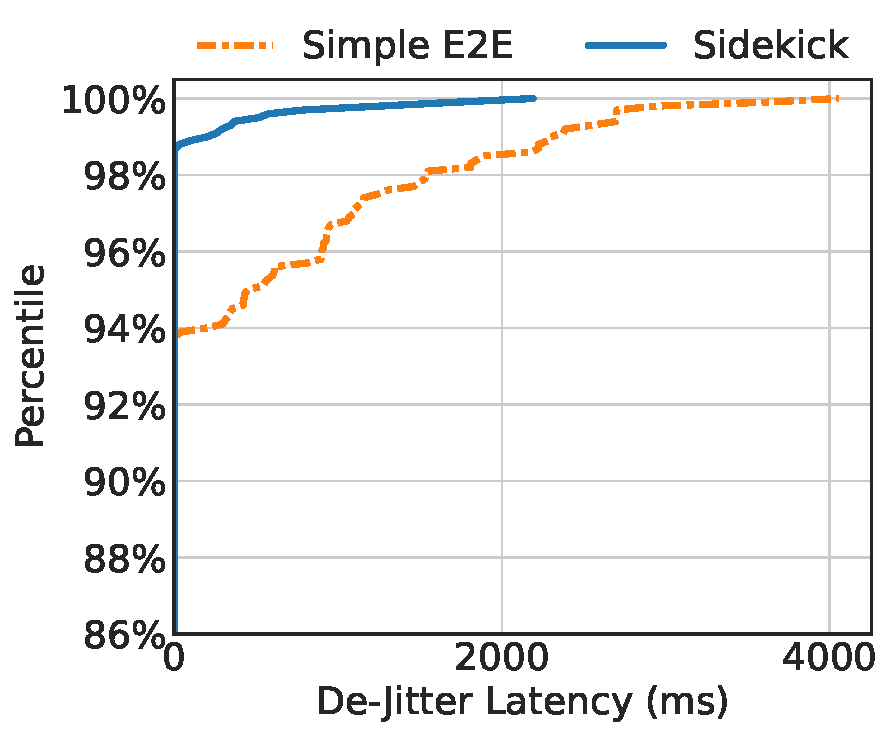
\includegraphics[width=\linewidth]{sidekick-paper/figures/fig8_real_world_webrtc.pdf}
	\caption{\footnotesize Low-latency media. CDF of per-packet de-jitter
	latencies over 10 one-minute trials per protocol.}
	\label{fig:real-world:scenario1}
\end{subfigure}
\begin{subfigure}{0.48\linewidth}
	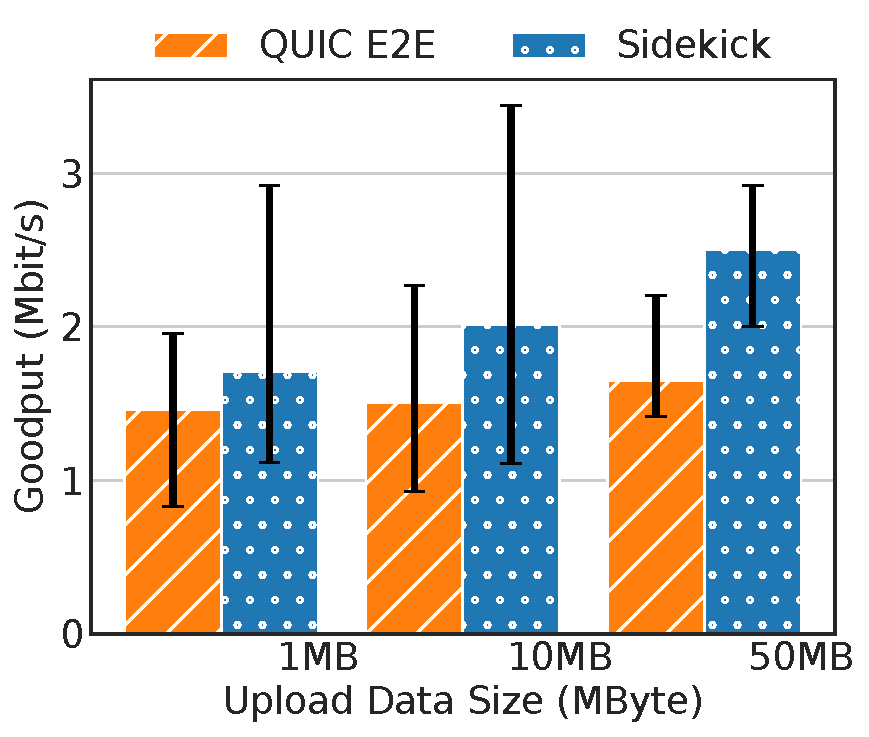
\includegraphics[width=\linewidth]{sidekick-paper/figures/fig8_real_world_retx.pdf}
	\caption{\footnotesize Path-aware congestion control.
	Median of 20 trials. Error bars are 1st and 3rd quartiles.}
	\label{fig:real-world:scenario2}
\end{subfigure}
\caption{Real-world results. Experiments were run in a moderately well-attended
office environment over a Friday afternoon. Trials alternate between the
baseline and the sidekick to account for variability in time of day.
}
\label{fig:real-world}
\end{figure}


We discuss the results of our experiments replicating two of our scenarios in
the real world, using as context
these main differences between emulation and the real-world:

% While we had controlled delays in emulation, in the real world they could
% be a lot more variable especially in the Wi-Fi link. But the delays on average
% were the same.
% The link between the client and the laptop AP resembled random loss that
% increased as we moved farther from the AP. Loss rates of $1$ to $10\%$ are
% reasonable to expect, depending on the distance. The loss was slightly more
% clustered, with XX clusters representing the first XX losses at $1\%$ loss.
% In emulation, this was XX clusters.
% The link between the cellular modem and the AWS server was mostly reliable.
% It was also the bottleneck link in terms of bandwidth.

\begin{itemize}[noitemsep,topsep=0pt]
	\item The RTT is more variable as it depends on interactions in the
	wireless medium and the shared cellular path.
	\item Wireless loss can be more variable as nearby 2.4 GHz devices and
	physical barriers may interfere with the link. Wireless loss also tends
	to be more clustered in practice.
	\item The available bandwidth on the shared cellular path is more variable,
	and depends on the time of day.
\end{itemize}

% real_world.py
%
% plot_retx_graph()
% bm = 'quic'
% ys = [1.4621363597978088, 1.5052205824076301, 1.651703594753664]
% bm = 'quack'
% ys = [1.7044382324644844, 2.0141072004377714, 2.504125876047309]
% 2.504125876047309 / 1.651703594753664 = 1.516
%
% plot_webrtc_graph()
% key = 'base'
% xs[190] = 99.0
% ys[190] = 2298.447371 ms
% key = 'quack'
% ys[190] = 204.465914
% 2298.447371 / 204.465914 = 11.241
\Cref{fig:real-world} shows the results of running the low-latency media and
connection-splitting PEP emulation experiments in the real-world. The baseline
protocol with a \sys is able to
reduce the 99th percentile de-jitter latency of an audio stream
from 2.3~seconds to 204~ms---about a 91\% reduction---and
improve the goodput of a 50 MB HTTP/3 upload by about 50\%.
Although the improvements are more conservative compared to emulation in
\Cref{fig:media} and \Cref{fig:baseline-line}, each case still benefits the
base protocol under all circumstances, compared to end-to-end mechanisms alone.

Part of the difference can be attributed to the network setting. When there is
no loss on the near path segment, as can occasionally happen in a real Wi-Fi link,
we do not expect to
see a difference with a \sys. When there is more loss on the far path segment, which
is variable and depends on the time, we
expect the benefit of the \sys to be less since this equally affects the
performance of the base protocol.

The other part of the difference could be made up by future work that better
adapts a \sys connection to real-world variability: The client could improve
path segment RTT estimation based on when the proxy receives packets, and use this
dynamic estimate in the calculation of $r$ used in $\beta$ and $C$.
The client could also use
this estimate to dynamically adjust the quACK interval.
Finally, we could analyze theoretically how PACUBIC responds
to traffic patterns in the real world.
